\documentclass[letterpaper,11pt]{article}
%--------------Document configuration begins--------------
\usepackage{fullpage}
\usepackage[numbers]{natbib} 	%\citet{jon90} --> Jones et al. [21], \citep{jon90} --> [21]
\usepackage[colorlinks]{hyperref}
%--------------Document configuration ends--------------

%Import personal commands 
\usepackage{commandscsp}		

%Load cleveref last
\usepackage{amsthm}
\usepackage[capitalize]{cleveref}
\usepackage{commands_theo} 			%Theorems, lemmas, proofs, etc

\title{\vspace{-1cm} \bf Constrained Shortest Path \vspace{-1.3cm}}
\author{}
\begin{document}
\maketitle


\section{Average HD}\label{sec:avg_hd}

The partial-witness property and \cref{theo:witness_doubling} provide a nice link between the CHD and HD, essentially showing that scaling CSP queries is of similar complexity to scaling SP queries as long as any efficient path contains large shortest-path segments. 
As an example, consider a \emph{multimodal mapping service} which gives transit routes combining walking, bus and subway, while ensuring at most $k$ transfers. 
For $k=3$, each route has at most $4$ segments, which gives use the partial witness property with $\beta = 2$. 
Now if each individual network has small HD, then the CHD is also small.

Converting the partial-witness condition to a more interpretable condition is difficult in general, as the structure of $\PS$ and $\PE$ may be complex. 
One way to get such a condition, however, is by considering \emph{average-case} performance metrics.
For this, we relax the definition of HD in two ways: $(i)$ we require LSHS to be locally sparse ``on average'' over all nodes, and
$(ii)$ we only require the existence of LSHS (as opposed to a hitting set for $S_r(v,\calQ)$).

\begin{definition}[Average LSHS]
Given $r>0$ and a system $\calQ$, a set $C\subseteq V$ is an average $(h,r)$-LSHS if it hits $\calQ_r$ and is locally sparse in average, i.e.,
$\frac{1}{n}\sum_{v\in V} \abs{B_{2r}(v)\cap C} \leq h$.
\end{definition}
\begin{definition}[Average HD]
The system $\calQ$ has average HD $h$ if, for every $r>0$, there exists an average $(h,r)$-LSHS.
\end{definition}

From the definition is clear that average HD is a strictly weaker property than HD; in particular, as we discuss before, the existence of LSHS does not guarantee their efficient computation.
Nevertheless, the above definition turns out to suffice to parametrize the average behavior of HL:
\begin{theorem}\label{theo:preproc_avg}
If $\PS$ has average HD $h$, then we can obtain, in polynomial time, HL with average size 
$\frac{1}{n}\sum_{v\in V} \abs{\Lf(v)} \leq h'\log D$ and 
$\frac{1}{n}\sum_{v\in V} \abs{\Lb(v)} \leq h'\log D$,
where $h'=\Or(\Delta h\log (hn\Delta))$.
\end{theorem}
Note that since query time depends linearly on the hub size, the above result implies both storage and performance bounds.
%\begin{proof}
%We only go over the preprocessing, since the construction is the same as in \cref{theo:construct_hl} and the bound for the size easily follows. 
%The objective is to obtain a set $C_i$ which is an average $(h',2^i)$-LSHS.
%This turns out to be a minimum cost hitting set problem.
%Indeed, we want to solve
%$
%\min\crl{\sum_{v\in V}\abs{B_{2r}(v)\cap C}: C\subseteq V, C \text{ hits } \PS_r}.
%$
%This follows from a symmetry argument, assigning to each node $u$ the cost $c(u)=\abs{\crl{v\in V: u\in B_{2r}(v)}}$.
%On the other hand, given a minimum cost hitting set problem with optimum value $\tau$, if the set system has VC-dimension $d$, the algorithm in \cite{vc_dim_hitting} finds a solution, in polynomial time, with cost at most $\Or(d\tau\log(d\tau))$.
%
%By assumption, the minimum of the problem is at most $hn$.
%Now we perform a mapping, where the ground set is changed to $E$ and paths are sequences of edges instead of nodes.
%This system still has VC-dimension 2, and now the minimum is at most $h\Delta n$.
%We apply the algorithm in \cite{vc_dim_hitting} and obtain a solution $C_i$ with cost at most $\Or(h\Delta n\log(h\Delta n))$; this gives the promised average $(h',r)$-LSHS.
%\end{proof}


\section{Relaxed Witness Property}\label{sec:rel_witness}

We describe a realistic setting where we can obtain small, in average, HL for the CSP.

First, we assume that individual edges are shortest paths, which is clearly true in road networks, and add an additional constraint wherein we insist our efficient paths have bounded \emph{stretch} compared to the shortest path; note that this is natural in applications as users do not want to be presented solutions which are far away from the optimum, even if it saves them budget.
Formally, we define:

\begin{definition}[Stretch]
	An algorithm for CSP has stretch $\St\geq 1$ if, $\forall s,t\in V$ and $b\leq B$, outputs $\dist(s,t|b)$ whenever $\dist(s,t|b)\leq \St\dist(s,t)$ and outputs ``infeasible'' when $\dist(s,t|b)>\St\dist(s,t)$.
\end{definition}
We henceforth input $\St$ as an extra constraint given by the application. 
Next, let $\Ec\defeq\crl{e\in E:c_e>0}$ denote the set of `costly' edges.
We define the following notion of an \emph{overpass}:

\begin{definition}[Overpass]
For $r>0$, the edge $e=(u,v)$ is an $r$-overpass if:\\
$(1)$ $e$ belongs to a path $Q\in\PE_{2r}\setminus\PS$\\
$(2)$ both $u$ and $v$ are endpoints of paths in $\PS_{r(2/\St-1)}$ and\\ 
$(3)$ $\min(\dist(e,\Ec),\dist(\Ec,e))\leq 3r/2$
\end{definition} 
Essentially, overpasses are edges connecting long shortest-paths in a costly zone; \cref{fig:overpass} shows an example. In case costs are contiguous (for example, tolls on highways or traffic jams), then the definition corresponds to the intuitive notion of an overpass.
Our main requirement is the following \emph{bounded growth} condition, controlling the number of $r$-overpasses for every scale $r>0$.

\begin{figure}[!b]
	\centering
	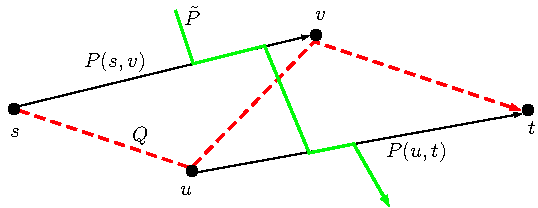
\includegraphics[scale=0.7]{TexImg/overpass.pdf}
	\caption{Edge $uv$ here is an overpass, lying on efficient path $Q$ (dashed red), connecting a pair of long shortest paths $P(s,v)$ and $P(u,t)$, and close to costly edges $\tilde P$ (solid green). } 
	\label{fig:overpass}
\end{figure}


\begin{definition}[Bounded Growth]
$(G,c,\ell)$ satisfies the bounded growth condition if, $\forall r>0$, $\abs{\crl{u\in V: \exists v, uv \text{ is an $r$-overpass}}}\leq \phi(2r)$, where $\phi(r)\defeq nh\alpha^{\beta-2-\log_2r}$
\end{definition}

Observe that $\phi$ is a slowly decreasing function of $r$ and, even when $r=D$, we allow for overpasses.
Now, with these conditions, we get our main result of this section:


\begin{theorem}\label{theo:overpasses}
Let $(G,\ell,c)$ be a network with HD $h$.
If the bounded growth is satisfied, we can obtain, in polynomial time, hub labels for CSP queries that guarantee average query-time $\Or((b+1)\alpha h'\log D)$ and total storage $\Or(nB\cdot B\alpha h'\log D)$, where $h'=\Or(\Delta h\log(hn\Delta))$.
\end{theorem}

We henceforth refer to the average HD of $\PE$ as average CHD.
Since the average HD is enough to obtain good preprocessing algorithms (cf. \cref{theo:preproc_avg}), an average CHD should intuitively suffice.
However, to prove \cref{theo:overpasses}, we need to show that it is possible to obtain small average CHD under even less restrictive assumptions than the partial-witness.
To do this, we first allow for an additional \emph{supplementary witness set} $D$ such that \emph{every efficient path is either witnessed by a shortest-path or hit by $D$}.
This corresponds to the intuition that a few bad efficient paths should not completely ruin the algorithm. 

\begin{definition}[Weak Partial Witness]
Given $\beta\geq 0$, we say a path system  $\calQ$ is weakly $\beta$-witnessed by the path system $\calQ'$ if, for every $r>0$, $\exists D_r\subseteq V$ such that, $\forall Q\in \calQ_r$ either (1) $Q$ is $\beta$-witnessed by $\calQ'$ or (2) $Q$ is hit by $D_r$.
Additionally we require $\abs{D_r}\leq \phi(r)$.
\end{definition} 

Intuitively, the supplementary witness set $D_r$ takes care of all the corner cases where $\calQ$ and $\calQ'$ differ too much.
We now show that our requirement on $\abs{D_r}$ guarantees a bound on the average HD.

\begin{proposition}\label[proposition]{prop:lay_witness}
Assume that $G$ is $\alpha$-doubling and let $\calQ'$ be weakly $\beta$-witnessed by $\calQ$.
If the HD of $\calQ$ is $h$, then the average HD of $\calQ'$ is $h'\leq 2\alpha^{\beta}h$
\end{proposition}
\begin{proof}
Let $r>0$, and $C$ be an $(h,2^{-\beta}r)$-LSHS for $\calQ$.
We show that $C\cup D_r$ is an average $(h,r)$-LSHS for $\calQ'$.
Clearly is a hitting set for $\calQ'_r$ and we can compute
\begin{align*}
h'&\leq \frac{1}{n}\sum_{v\in V} \abs{B_{2r}(v)\cap (C\cup D_r)}\\
&\leq \frac{1}{n}\prn*{\sum_{v\in V} \abs{B_{2r}(v)\cap C}+\sum_{v\in V} \abs{B_{2r}(v)\cap D_r}}\\
&\leq \frac{1}{n}\prn*{\sum_{v\in V} \alpha^\beta h+\sum_{v\in D_r} \abs{B_{2r}(v)}}
\leq \alpha^\beta h + \frac{\abs{D_r}\alpha^{\log_2r+2}}{n}.
\end{align*}
In the third inequality we used that $C$ is sparse with respect to balls of radius $2^{-\beta+1}r$ and that $\sum_{v\in V} \abs{B_{2r}(v)\cap D_r}=\sum_{v\in D_r} \abs{B_{2r}(v)}$ by symmetry of the bi-directional balls.
In the last inequality we used that, by doubling dimension, balls of radius $r$ have at most $\alpha^{\log_2r+1}$ elements.
Since $\abs{D_r}\leq \phi(r)$, the result follows.
\end{proof}

This now allows us to link $\PE$ and $\PS$ as follows:
\begin{proposition}\label[proposition]{prop:1witness}
Under the bounded growth condition, $\PS$ is a weak $1$-witness for $\PE$.
\end{proposition}
\begin{proof}
We first need some additional notation:
For a path $Q$ and two vertices $u,v\in Q$ we denote $Q[u,v]\subseteq Q$ as the sub $(u,v)$-path; for two paths $P,Q$ with a common endpoint, we denote $P|Q$ as their concatenation.

Consider $Q\in\PE$ with endpoints $s,t$ and set $\ell(Q)=2r$.
We will show how to obtain a vertex for the supplementary witness set in case $Q$ is not witnessed and then we bound the size of the set.
Assume that $Q\neq P(s,t)$, otherwise the path is trivially witnessed.
Let $(u,v)\in Q$ be such that $\ell(Q[s,v]),\ell(Q[u,t])\geq r$. 
If either $Q[s,v]$ or $Q[u,t]$ is a shortest path or $\ell_{uv}\geq r$, then $Q$ is witnessed. Thus, we henceforth assume that all of the above conditions fail.

We claim that $uv$ is a $r$-overpass (in fact, this is the exact scenario depicted in \cref{fig:overpass}).
Condition 1 is clearly satisfied. 
Condition 2 also holds because both $Q[s,v]$ or $Q[u,t]$ have stretch at most $\frac{2-\St}{\St}$.
To see this, note that both $P(s,v)|Q[v,t]$ and $Q[s,u]|P(u,t)$ are no shorter than $P(s,t)$ and $\St\ell(P(s,t))\geq \ell(Q)$, hence
$\frac{2r}{\St}\leq \ell(P(s,t)) \leq  \ell(P(s,v)) + \ell(Q[v,t])$ and $\frac{2r}{\St} \leq \ell(P(s,t)) \leq  \ell(Q[s,u]) + \ell(P(u,t))$.
Since each path $Q[s,u],Q[v,t]$ has length less than $r$, it follows that both $P(s,v),P(u,t)$ have length strictly greater than $\frac{2-\St}{\St}r$. % and condition 1 follows. 
Finally, to show condition 3, we have $\ell(Q[s,v])+\ell(Q[u,t])=r+\ell_{uv}$ and since $\ell_{uv}<r/2$, one of $Q[s,v]$ or $Q[u,t]$ has length at most $3r/4$.
Since neither of these paths is shortest, it must be that both $P(s,v),P(u,t)$ have costly edges and thus one of $u,v$ is closer than $3r/4$ to $E_1$ and the condition is satisfied.

For every path of length $2r$, we can thus either exhibit a witness or show that it contains an overpass and add use the tail of the edge as a supplementary witness.
For a fixed $r>0$, we need to add at most $\phi(r)$ nodes to $D_r$ to cover all the efficient paths. 
The result follows.
\end{proof}

We are almost ready to prove that bounded growth allows to solve the CSP.
The last piece is \cref{prop:avg_chd}, the proof of which follows form similar arguments as those in \cref{theo:HLeff,theo:preproc_avg}.

\begin{proposition}\label[proposition]{prop:avg_chd}
If the average HD of $\PE$ is $h_c$, then we can construct, in polynomial time, hub labels for CSP, which guarantee average query-time $\Or((b+1)h_c'\log D)$ for queries with budget $b$, and total storage requirements $\Or(nB\cdot Bh_c'\log D)$.
\end{proposition}

\begin{proofof}{\cref{theo:overpasses}}
We argue that the average CHD is $h_c\leq 2\alpha h$.
By \cref{prop:1witness}, $\PE$ is weakly $1$-witnessed by $\PS$.
It follows by \cref{prop:lay_witness} that the average CHD is at most $2\alpha h$ as needed.
Applying \cref{prop:avg_chd} yields the result.
\end{proofof}

\section{Generalization to general constraint}

We have dealt with cost constraints so far, but our approach can be applied to more general settings.
Consider when edges have capacity instead of cost and we want the shortest path given a minimum capacity.
Another example is when edges have labels, e.g. if it is a carpool lane or not, if it is a main street, etc.
In the last example, we would like a shortest path avoiding certain labels, e.g. avoiding carpool lanes if the user travels alone.
We need to abstract the problem to obtain the connection between all these scenarios.

Given a path system $\calQ$, we want to find the shortest path among those in $\calQ$.
We assume that queries are in the form $(s,t,\calQ')$, where $s,t\in V$ and $\calQ'\subseteq\calQ$.
For example, the CSP has $\calQ=\PE$ and $\calQ'$ is the set of efficient paths with cost at most $b$.
The problem to solve is then $\min \ell(P) \text{ s.t. } P\in\Pst\cap\calQ'$ for an input $(s,t,\calQ')$.
We do not ask to solve for any input $\calQ'\subseteq \calQ$, but for \emph{admissible inputs}, which are defined by the designer.
For example, admissible inputs for the CSP are ``paths with cost at most $b$'', but ``paths with cost between $b_1$ and $b_2$'' are not.  

\begin{definition}[Integer Embedded Constraints]
Let $\calQ$ be any path system.
If there is a function $\psi:\calQ\to\Z^d$ such that, for any admissible input $\calQ'\subseteq \calQ$, $\exists b\in \Z^d$ with the property $P\in \calQ'\Leftrightarrow \psi(P)\leq b$, then we say that $\psi$ is an integer embedding of the problem.
\end{definition}

\begin{proposition}
The following are integer embedded constraints \anote{the definition of efficient depends on the problem}
\begin{enumerate}
\item CSP, with $\calQ=\crl{P\in \PE: c(P)\leq B}$ for a given $B$. 
The function is $\psi(P)=c(P)$ and $b$ is the natural choice.
\item Capacity constraints, with $\calQ=\crl{P\in \PE: \text{cap}(P)\leq B}$ for a given $B$.
The function is $\psi(P)=\min_{e\in P}\text{cap}(P)$ and $b$ is the minimum capacity.
\item Label constraints with $\calQ=\crl{P\in \PE: \text{labels}(P) \in B}$ for a given $B\subseteq 2^{\text{Labels}}$.
In this case the dimension is $\abs{\crl{l:l\text{ is in an element of }B}}$ and $\psi(P)_l = \In{P \text{ has label }l}$.
\item CSP with pairwise correlated costs. In this case the dimension is two \anote{ to do }
\end{enumerate}
\end{proposition}


\begin{proposition}
If $\calQ$ has HD $h$ and has an integer embedding $\psi:\calQ\to\Z^d$, let $M=\max_i\max\crl{\psi(P)_i:P \text{ is admissible}}$.
Then, we can construct HL to answer queries in time $\Or(bh\log D)$.
The total space requirement is $\Or(nM\cdot Mh\log D)$.
\end{proposition}

\section{Examples}

An important notion is that, if efficient paths oscillate too much between free and tolled edges, then it is very unlikely to observe partial witnesses.
In Figure~\ref{fig:nosubpath} we present a graph with no $\frac{1}{2}$-partial witness.
Every edge has unit length, dash edges have zero cost and solid edges have unit cost.
The path $uvwx$ is efficient, but every subpath that is shortest has length one.
The example can be generalized by placing the graph side by side many times.
This shows that, for any constant $k$ we can find examples with no $\frac{1}{k}$-partial witnesses.


\begin{figure}
\caption{Example with unit cost and no subpath property}
\label{fig:nosubpath}
\centering
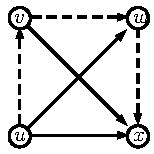
\includegraphics[scale=1.3]{TexImg/Nosubpath.pdf}
\end{figure}

\bibliographystyle{plainnat}
\bibliography{biblio}

\end{document}
